% ---- pg-021 （书页 9） ----

图,它们可以从原始观测值直接得到,也可将点投影到散布图的每个坐标轴上得到.

单变量点图中所包含的信息可被用来计算样本均值 $\bar{x}_1$ 和 $\bar{x}_2$ 及样本方差 $s_{11}$ 和 $s_{22}$(参考练习 1.1.)散布图表明了点的方位,这些点的坐标可用来计算样本协方差 $s_{12}$.在\hyperref[fig:1.1]{图 1.1} 的散布图中,$x_1$ 的大值与 $x_2$ 的大值一起出现,而 $x_1$ 的小值与 $x_2$ 的小值一起出现.因此,$s_{12}$ 将是正的.

点图与散布图包含了不同类型的信息.边缘点图中所含信息不足以构造出散布图.作为一个说明,假设对前面\hyperref[fig:1.1]{图 1.1} 中的数据重新配对之后,使得变量 $x_1$ 和 $x_2$ 的测量值如下:

变量 1$(x_1)$: \quad 5 \quad 4 \quad 6 \quad 2 \quad 2 \quad 8 \quad 3

变量 2$(x_2)$: \quad 5 \quad 5.5 \quad 4 \quad 7 \quad 10 \quad 5 \quad 7.5

(我们已简单地重新排列了变量 1 的数值.)数据重新排列过的散布图和点图如\hyperref[fig:1.2]{图 1.2} 所示.比较\hyperref[fig:1.1]{图 1.1} 和\hyperref[fig:1.2]{图 1.2},我们发现边缘点图是相同的,而散布图却明显不同了.在\hyperref[fig:1.2]{图 1.2} 中,$x_1$ 的大值与 $x_2$ 的小值一起出现,而 $x_1$ 的小值又与 $x_2$ 的大值同时出现.因此,描述统计量中单独的变量 $\bar{x}_1,\bar{x}_2,s_{11}$ 和 $s_{22}$ 保持不变,而度量一对变量间结合的样本协方差 $s_{12}$ 现在却变为负数.

\begin{mvfigure}
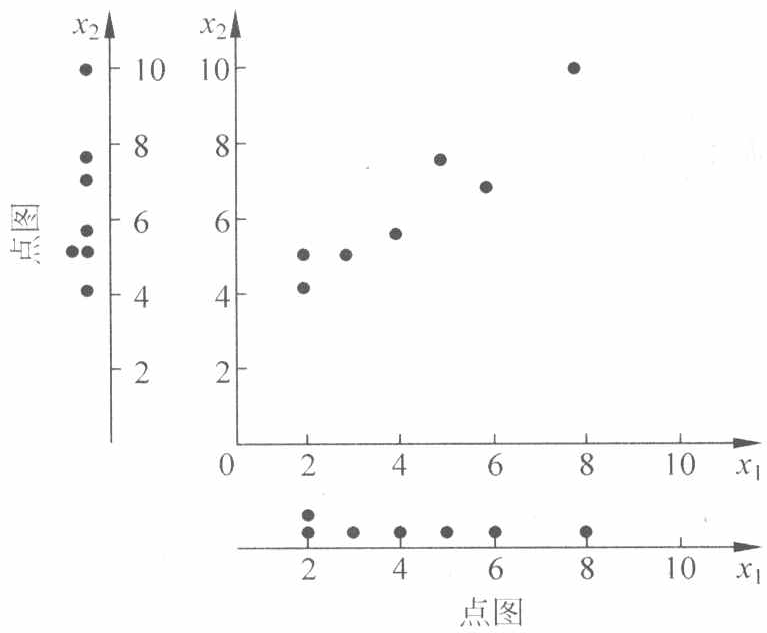
\includegraphics[width=\mvimgw]{figs/fig_pg021_1.png}
\phantomsection\label{fig:1.1}\mvcap{图 1.1\quad 散布图和边缘点图}
\end{mvfigure}

\begin{mvfigure}
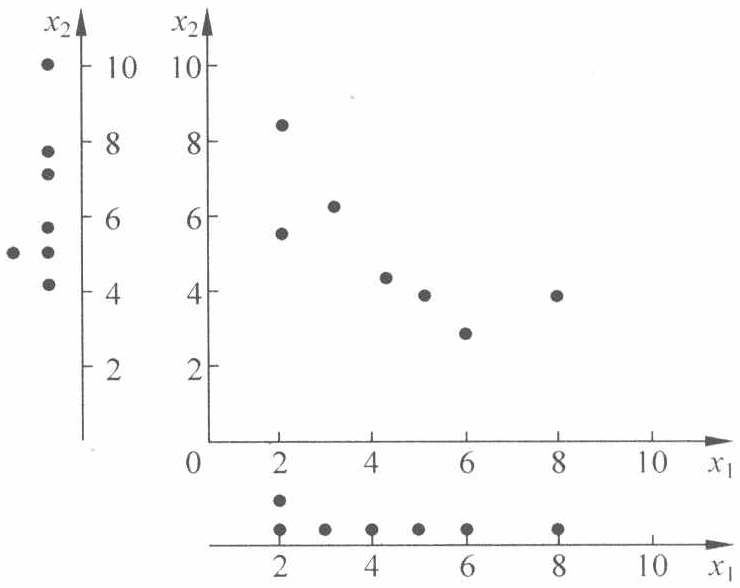
\includegraphics[width=\mvimgw]{figs/fig_pg021_2.png}
\phantomsection\label{fig:1.2}\mvcap{图 1.2\quad 数据重新排列后的散布图和点图}
\end{mvfigure}

\hyperref[fig:1.1]{图 1.1} 和\hyperref[fig:1.2]{图 1.2} 中数据的不同取向无法通过单独的边缘点图辨别.然而,在两种情况下边缘点图是相同的,这个事实也无法立即从散布图中显示出来.这两种图解法不是对立的,而是相互补充的.

接下来两个例子可进一步说明通过图形表示可以传递的信息.

\mvbold{例 1.3}\quad (异常的观测值对样本相关系数的影响)

\begin{mvfigure}
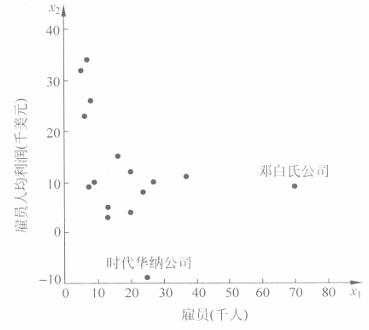
\includegraphics[width=\mvimgw]{figs/fig_pg021_fig13.png}
\phantomsection\label{fig:1.3}\mvcap{图 1.3\quad 16 家出版公司的雇员人均利润和雇员人数}
\end{mvfigure}

% ---- 以下内容在源 PDF 中已损坏丢失（书页 9 图像自页高约 68\% 处截断）----
% 已依据用户提供的同一扫描件完好副本（clipboard-2026-10-04）补齐：
%   1) 正文一段："接下来两个例子可进一步说明通过图形表示可以传递的信息." + 例 1.3 标题
%   2) \hyperref[fig:1.3]{图 1.3}（纵轴"利润(千美元)"、刻度 20/30/40；数据点旁标注"邓白氏公司"）
% 来源：用户提供的同一扫描件完好副本（原书书页 9 对应页）
% UNCERTAIN: \hyperref[fig:1.3]{图 1.3} 的图题（caption）与下文在损坏区域中，未见；待用户补充后核对。

